% !TEX TS-program = xelatex
% !TEX encoding = UTF-8 Unicode
\documentclass[11pt,a4paper]{article}
\usepackage{amsmath,amssymb}
\usepackage{empheq}
\usepackage[semibold]{ebgaramond}
\usepackage[cmintegrals,cmbraces]{newtxmath}
\usepackage{ebgaramond-maths}
\usepackage{bm}
\usepackage[OMLmathrm, OMLmathsfit, rmdefault=mdugm]{isomath}
\usepackage{tocbibind}
\usepackage{graphicx}
\graphicspath{{./pics/}}
\usepackage{wrapfig}
\usepackage{capt-of}

\makeatletter
  \DeclareSymbolFont{ntxletters}{OML}{ntxmi}{m}{it}
  \SetSymbolFont{ntxletters}{bold}{OML}{ntxmi}{b}{it}
  \re@DeclareMathSymbol{\leftharpoonup}{\mathrel}{ntxletters}{"28}
  \re@DeclareMathSymbol{\leftharpoondown}{\mathrel}{ntxletters}{"29}
  \re@DeclareMathSymbol{\rightharpoonup}{\mathrel}{ntxletters}{"2A}
  \re@DeclareMathSymbol{\rightharpoondown}{\mathrel}{ntxletters}{"2B}
  \re@DeclareMathSymbol{\triangleleft}{\mathbin}{ntxletters}{"2F}
  \re@DeclareMathSymbol{\triangleright}{\mathbin}{ntxletters}{"2E}
  \re@DeclareMathSymbol{\partial}{\mathord}{ntxletters}{"40}
  \re@DeclareMathSymbol{\flat}{\mathord}{ntxletters}{"5B}
  \re@DeclareMathSymbol{\natural}{\mathord}{ntxletters}{"5C}
  \re@DeclareMathSymbol{\star}{\mathbin}{ntxletters}{"3F}
  \re@DeclareMathSymbol{\smile}{\mathrel}{ntxletters}{"5E}
  \re@DeclareMathSymbol{\frown}{\mathrel}{ntxletters}{"5F}
  \re@DeclareMathSymbol{\sharp}{\mathord}{ntxletters}{"5D}
  \re@DeclareMathAccent{\vec}{\mathord}{ntxletters}{"7E}
\makeatother

\usepackage{array}
\usepackage{enumitem}
% to produce a comma between multiple footnotes / https://tex.stackexchange.com/questions/40072/incompatibility-between-footmisc-option-multiple-and-hyperref/62091#62091
\let\oldFootnote\footnote
\newcommand\nextToken\relax
\renewcommand\footnote[1]{%
    \oldFootnote{#1}\futurelet\nextToken\isFootnote}
\newcommand\isFootnote{%
    \ifx\footnote\nextToken\textsuperscript{,}\fi}

\defaultfontfeatures{Ligatures=TeX} % makes this a feature for all selected fonts
\usepackage{esint}
\usepackage{polyglossia}
\setmainlanguage{english}
\usepackage[text={18cm,26cm},centering]{geometry} % 
\usepackage{natbib}
\usepackage{mdframed}
\usepackage{lipsum}
\usepackage[usenames,dvipsnames,svgnames,table]{xcolor}
\usepackage{hyperref}
\usepackage{url}
\usepackage[export]{adjustbox}

\hypersetup{
  colorlinks,
  citecolor=bleuSU,
  linkcolor=bleuSU
}
\definecolor{bleuSU}{RGB}{26,39,101}

\usepackage[normalem]{ulem}
\makeatletter
\renewcommand*{\uuline}{%
  \bgroup
  \UL@setULdepth
  \markoverwith{%
    \lower\ULdepth\hbox{%
      \kern-.03em%
      \vtop{%
        \hrule width.2em%
        \kern 0.6pt % distance between the two underlines
        \hrule
      }%
      \kern-.03em%
    }%
  }%
  \ULon
}
\makeatother
\setlength{\ULdepth}{-2pt}  % distance from double underline to letter

\usepackage{environ}
\newtoggle{corrige}

\NewEnviron{answer}{%
  \iftoggle{corrige}
    {\begin{mdframed}\textbf{Answer: } \BODY\end{mdframed}}
    {}%
  }

\newcommand{\delS}{\delta S}
\newcommand{\delA}{\delta A}
\newcommand{\delh}{\delta h}
\newcommand{\delt}{\delta t}
\newcommand{\delz}{\delta z}
\newcommand{\delbx}{\delta \matrixsym x}
\newcommand{\lp}{\left(}
\newcommand{\rp}{\right)}
\newcommand{\itA}{\textit A}
\newcommand{\itB}{\textit B}
\newcommand{\dAB}{\mathcal D_{AB}}
\newcommand{\bA}{\matrixsym A}
\newcommand{\bff}{\matrixsym{f}}
\newcommand{\bF}{\matrixsym{F}}
\newcommand{\bj}{\matrixsym{j}}
\newcommand{\bJ}{\matrixsym J}
\newcommand{\bn}{\matrixsym{n}}
\newcommand{\bN}{\matrixsym N}
\newcommand{\bP}{\matrixsym{P}}
\newcommand{\br}{\matrixsym r}
\newcommand{\bt}{\matrixsym t}
\newcommand{\be}{\matrixsym e}
\newcommand{\bu}{\matrixsym u}
\newcommand{\bv}{\matrixsym v}
\newcommand{\bw}{\matrixsym w}
\newcommand{\bx}{\matrixsym x}
\newcommand{\pd}[2]{\frac{\partial #1}{\partial #2}}
\newcommand{\D}[2]{\frac{D #1}{D #2}}
\newcommand{\dd}[2]{\frac{\mathrm d #1}{\mathrm d #2}}
\newcommand{\dA}{\mathrm dA}
\newcommand{\dV}{\mathrm dV}
\newcommand{\dS}{\mathrm dS}
\newcommand{\prg}[1]{\paragraph{$\rhd$ #1}}
\newcommand{\alphaijkl}{\alpha_{ijkl}}
\newcommand{\Aijkl}{A_{ijkl}}
\newcommand{\delij}{\delta_{ij}}
\newcommand{\sigij}{\sigma_{ij}}
\newcommand{\sigji}{\sigma_{ji}}
\newcommand{\sigxy}{\sigma_{xy}}
\newcommand{\matL}{\mathcal L}
\newcommand{\matO}{\mathcal O}
\newcommand{\matS}{\mathcal S}
\newcommand{\kij}{k_{ij}}
\newcommand{\tensor}[1]{\smash{\uuline{#1}{}}}
\setlength{\parindent}{0pt} % remove indent

\setlist[enumerate]{topsep=0pt,itemsep=-1ex,partopsep=1ex,parsep=1ex}

\begin{document}
\setlength{\unitlength}{1cm}
\noindent
\parbox{\textwidth}{
\textsc{
Sorbonne Université  
\hfill
Year 2022-2023
}
}
\parbox{\textwidth}{
\textsc{
Faculté des Sciences
\hfill
Physics of Fluids \& Nonlinear Physics
}
}

\begin{center}
\Large
\textbf{Hydrodynamics} \\ 
\textsl{Tutorial 2: boundary conditions, capillarity \& adhesion} \\[1ex]
\end{center}

\section{Impermeable obstacles}
\togglefalse{corrige}

\begin{figure}[ht]
    \centering
    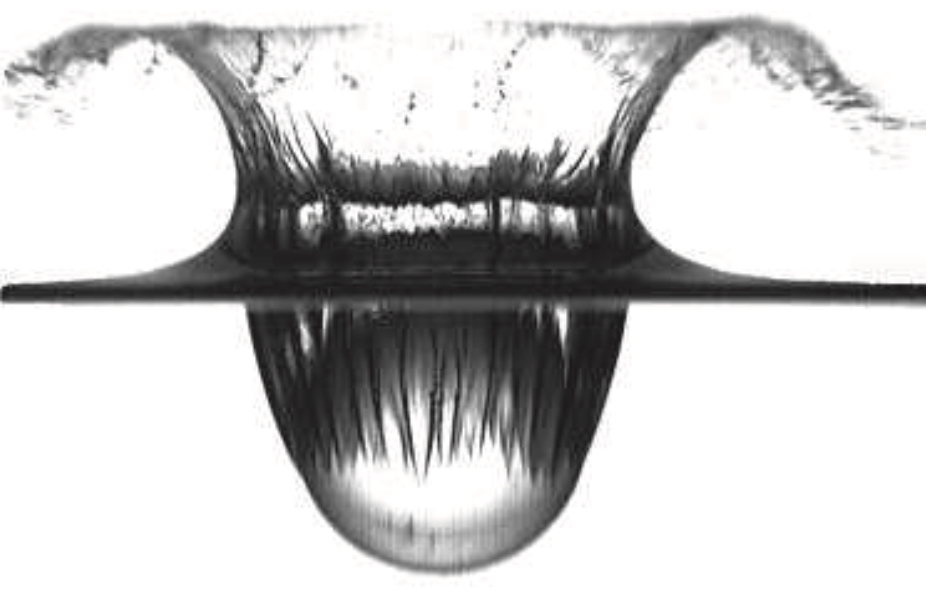
\includegraphics[height=3cm,valign=m]{splash.jpg}
    \hspace{1cm}
    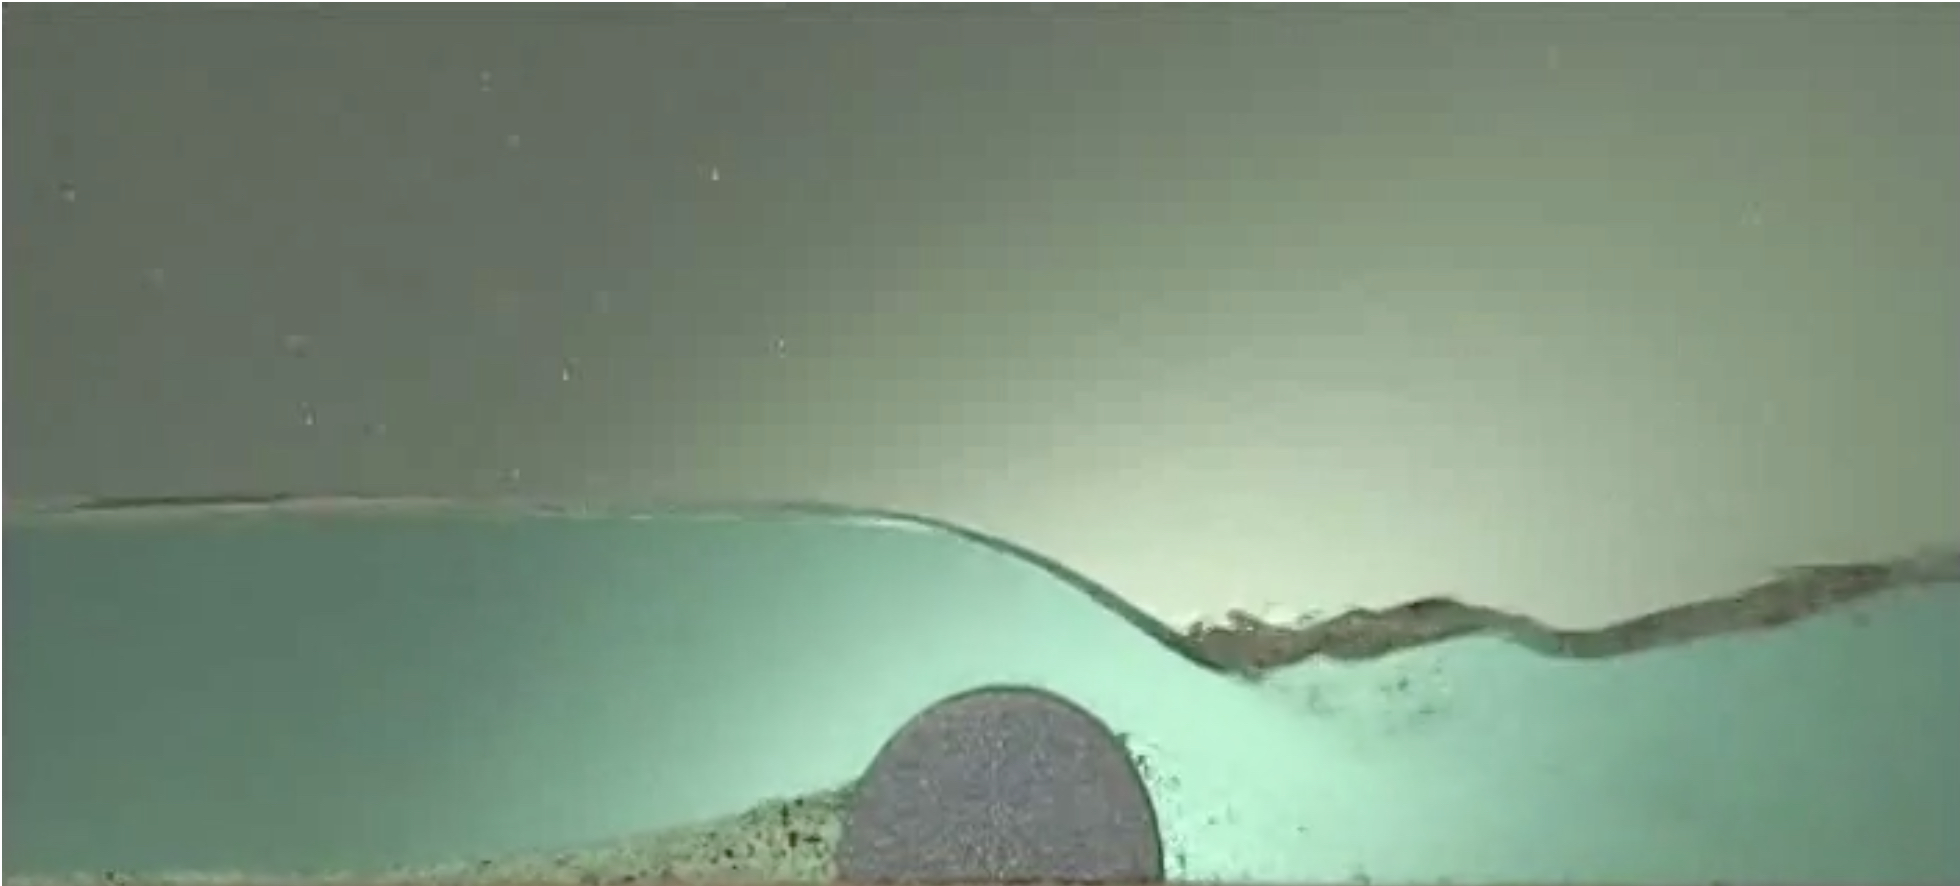
\includegraphics[height=3cm,valign=m]{flow_over_weir.jpg}
    \caption[Caption for LOF]{\textbf{Liquid deflection.} Left: an hydrophobic bead impacts a water pool at $\simeq 5$ m$\cdot$s$^{-1}$ and produces a splash (liquid corolla) on impact \citep{Eggers2007}. Right: a flow over an obstacle in a wave tank givers rise to the \textit{hydraulic jump} phenomenon (Science Education Resource Center at Carleton College\setcounter{footnote}{0}\footnotemark).}
    \label{fig:obstacle}
\end{figure}
\footnotetext{\url{https://serc.carleton.edu/NAGTWorkshops/geomoph/emriver/index.html}}
\prg{Impact.}
A spherical obstacle of radius $R$ impacts a liquid tank at velocity $-U_\text{impact} \be_{z}$. On impact the fluid is violently set into motion by the object.
\begin{enumerate}
\item Supposing that the object preserves its velocity during impact, determine the position $C$ of the sphere centre through time. Consider that at initial time $t=0$, $C$ is located at $(x,y,z)=(0,0,0)$. Deduce the equation of the sphere surface for all time in the laboratory (i.e. fixed) frame.
\item Obtain the expression for the normal vector $\bn$ at each point of the sphere in cartesian ccoordinates.
\item Noting the fluid velocity $\bu=(u,v,w)$, determine the expression for the impermeability condition at the sphere surface.
\begin{answer}
\begin{equation*}
ux+vy+w(z+U_\text{impact}t) = -U_\text{impact}(z+U_\text{impact}t)
\end{equation*}
\end{answer}

\end{enumerate}
\prg{Flow over an obstacle.} We now consider the flow of a river over an obstacle, such as the one illustrated~\ref{fig:obstacle}. For simplification purposes, we take the flow as uniform far upstream, $\bu = U \be_x$, and translation invariant (that is, 2D) in the transverse direction. The vertical direction is given by $\be_y$ and we note the velocity components $\bu=(u,v)$. The bottom height is given by the function $y = f(x)$. 
\begin{enumerate}[resume]
\item Determine the vector normal to the river bottom.
\item Express the impermeability condition at the bottom.
\begin{answer}
\begin{equation*}
v = u f'(x)
\end{equation*}
\end{answer}

\item Sketch schematically the vertical velocity near the bottom in the context of the localised obstable (think of a Gaussian hump). Comment.
\end{enumerate}
\section{Flow around a cylinder with suction}
We consider in this exercise the structure of the flow around a cylinder able to exert a suction (or blowing) on the surrounding fluid, as a rudimentary model of a \textit{turbosail} (see lecture).
\begin{figure}[ht]
    \centering
    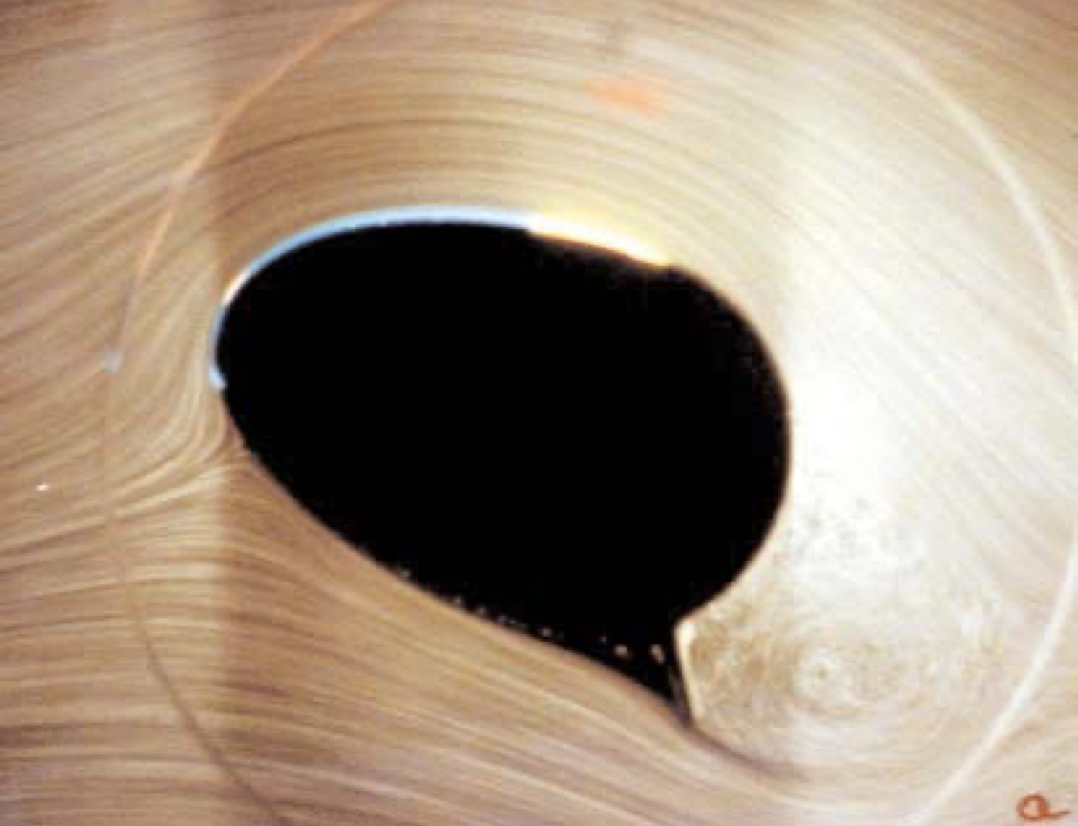
\includegraphics[height=5cm,valign=m]{aspiration_cylindre.jpg}
    \caption{\textbf{Turbosail model at ONERA.} The suction through the cylinder boundary allows the flow to reattach on the cylinder.}
    \label{fig:turbosail}
\end{figure}

In the remaining, we consider the flow as translation-invariant (2D), incompressible and potential. We note $\bu = (u,v)$ the components of the velocity field and we introduce the streamfunction $\psi$ such that:
\begin{empheq}[left=\empheqlbrace]{alignat=2}
u &\,=\,&\, \pd{\psi}{y} \\
v &\,=\,&\, -\pd{\psi}{x}
\end{empheq}
Depending on the context we will use cartesian coordinates $(x,y)$ or polar ones $(r,\theta)$.
\begin{enumerate}
\item Show that a flow describe with such a streamfunction automatically satisfies mass conservation.
\begin{answer}
If the flow is incompressible then mass conservation reduces to:
\begin{equation*}
\nabla \cdot \bu = 0.
\end{equation*}
For a flow described by a streamfunction the velocity field divergence reads:
\begin{equation*}
\nabla \cdot \bu = \pd{}{x}\lp\pd{\psi}{y}\rp-\pd{}{y}\lp\pd{\psi}{x}\rp = 0
\end{equation*}
by construction, whatever $\psi$.
\end{answer}
\item Show that the potential flow condition implies $\Delta \psi = 0$.
\begin{answer}
A potential flow is such that:
\begin{equation*}
\nabla \times \bu = 0.
\end{equation*}
For a 2D flow this condition reduces to: 
\begin{equation*}
\pd{v}{x}-\pd{u}{y} = 0.
\end{equation*}
On using the relation between $(u,v)$ and $\psi$ we get $-\Delta \psi =0$.
\end{answer}
\item Verify that $\psi_\text{unif} = a y$ and $\psi_\text{source} = b\theta$ are elementary solutions of $\Delta \psi = 0$. What are the associated flow patterns?
\begin{answer}
These two streamfunctions are linear in $y$ and $\theta$, and thus verify Laplace equation trivially.

{\centering
      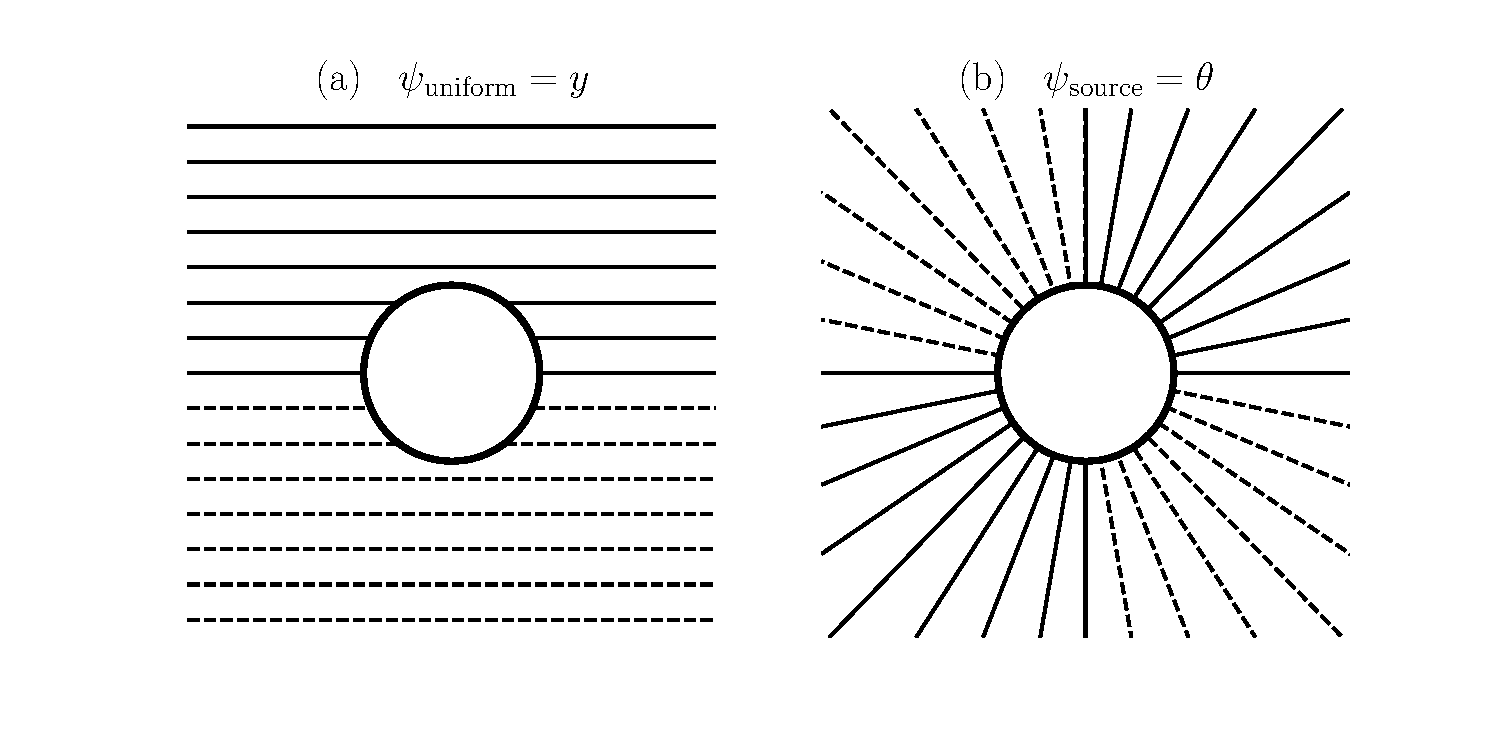
\includegraphics[width=12cm]{uniform_source.pdf}
      \captionof{figure}{Left: the isolines for $\psi_\text{uniform}$ evidence a uniform flow. Right: the isolines for $\psi_\text{source}$ show the purely radial flow typical of a \textit{source}.}
      \par}
\end{answer}
\item What is the streamfunction associated with a uniform flow $\bu = (U,0)$ ?
\begin{answer}
We have directly:
\begin{equation*}
\psi = Uy
\end{equation*}
\end{answer}
\item More complex multipolar solutions can be built from the previous elementary solutions. Compute the expression for the dipolar fields $\psi_{\parallel} = \pd{}{x} \psi_\text{source}$ and $\psi_{\perp} = \pd{}{y} \psi_\text{source}$. Represent the corresponding streamlines with Python.
\begin{answer}
Let's write $\psi_\text{source}$ in cartesian coordinates:
\begin{equation*}
\psi_\text{source} = \arctan\lp\frac{y}{x}\rp.
\end{equation*}
Using $\partial_x\lp\arctan\lp f \rp \rp=\frac{\partial_x f}{1+f^2}$ we have:
\begin{empheq}[left=\empheqlbrace]{alignat=2}
\psi_{\parallel}  \,&=&\, -\frac{y}{r^2}\\
\psi_{\perp} \,&=&\, \frac{x}{r^2}
\end{empheq}
{\centering
      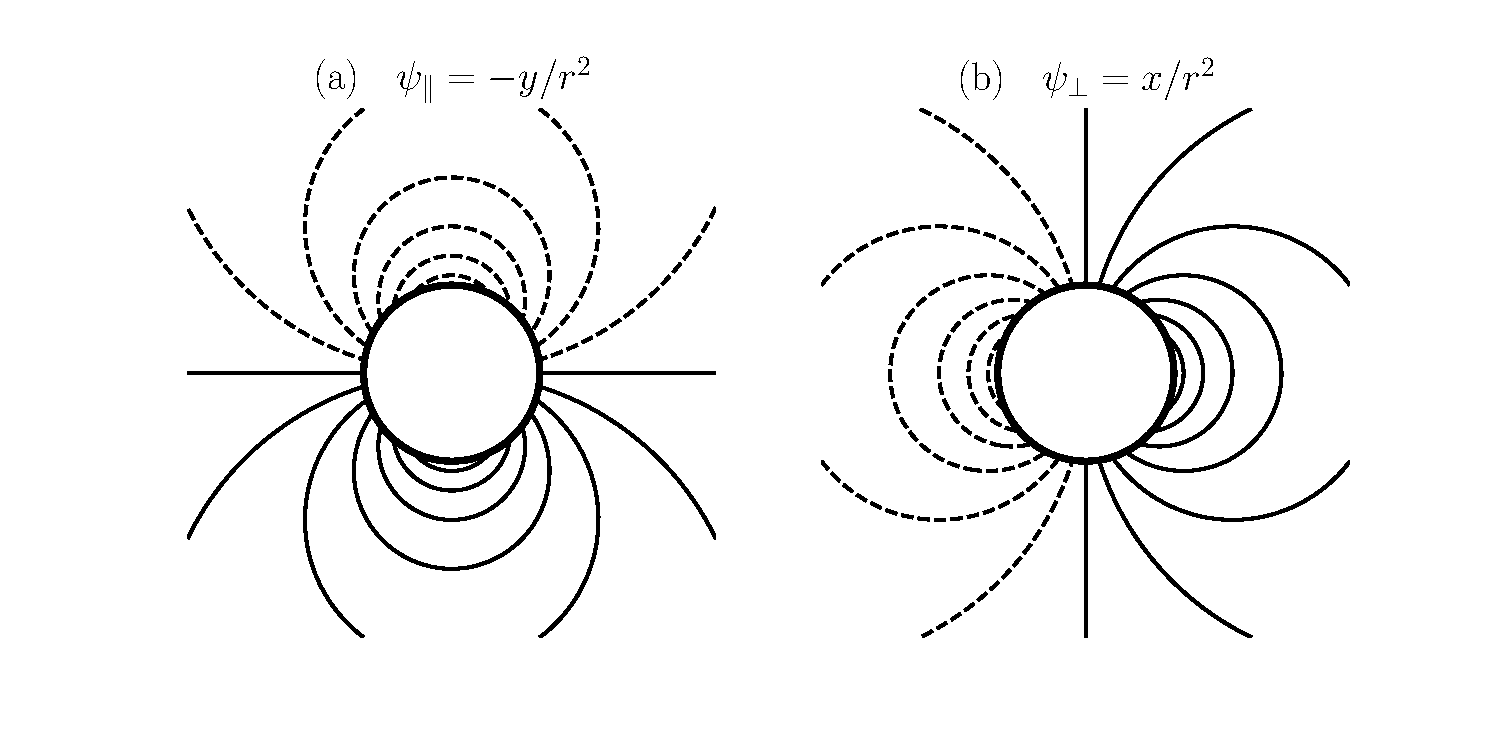
\includegraphics[width=12cm]{psi_dipoles.pdf}
      \captionof{figure}{Left: $\psi_\parallel$. Right: $\psi_\perp$.}
      \par}
\end{answer}
\item Show that it is possible to build the inviscid potential flow around a cylinder of radius $R$ as the superposition of  $\psi_\text{unif}$ and of a dipolar contribution.
\begin{answer}
The impermeability condition on the cylinder reduces to $\psi = \text{cst}$ along its surface, that is on $r = R$. The only way to fulfill this condition with a streamfunction of the form
$$
\psi = \psi_\text{unif}  + a \psi_{\parallel} + b \psi_{\perp} = Uy - a \frac{y}{r^2} + b \frac{x}{r^2}
 $$
is to set $a = U R^2$ and $b = 0$.
\end{answer}
\item Propose a model for the suction effect, which is characterised with a constant suction velocity  $- u_\text{suction} \be_r$ at the wall.
\begin{answer}
The flow associated to $\psi_\text{source}$ is purely radial and can be represented as:
$$
\bu_\text{source} = \frac{x}{r^2} \be_x + \frac{y}{r^2} \be_y.
$$
At the cylinder surface,
$$
\left.\bu_\text{source}\cdot\bn\right|_{r=R} = \frac{1}{R}.
$$
In order to impose a wall velocity $- u_\text{suction} \be_r$ we need to add the following streamfunction
$$
\psi_\text{suction} = - u_\text{suction} R \theta
$$
\end{answer}
\item Represent with Python the streamlines corresponding to $u_\text{suction} / U = 0, 0.1, 1$.
\begin{answer}
We represent the streamlines associated to:
$$
\psi = Uy - U R^2  \frac{y}{r^2} - u_\text{aspi} R \theta
$$
{\centering
      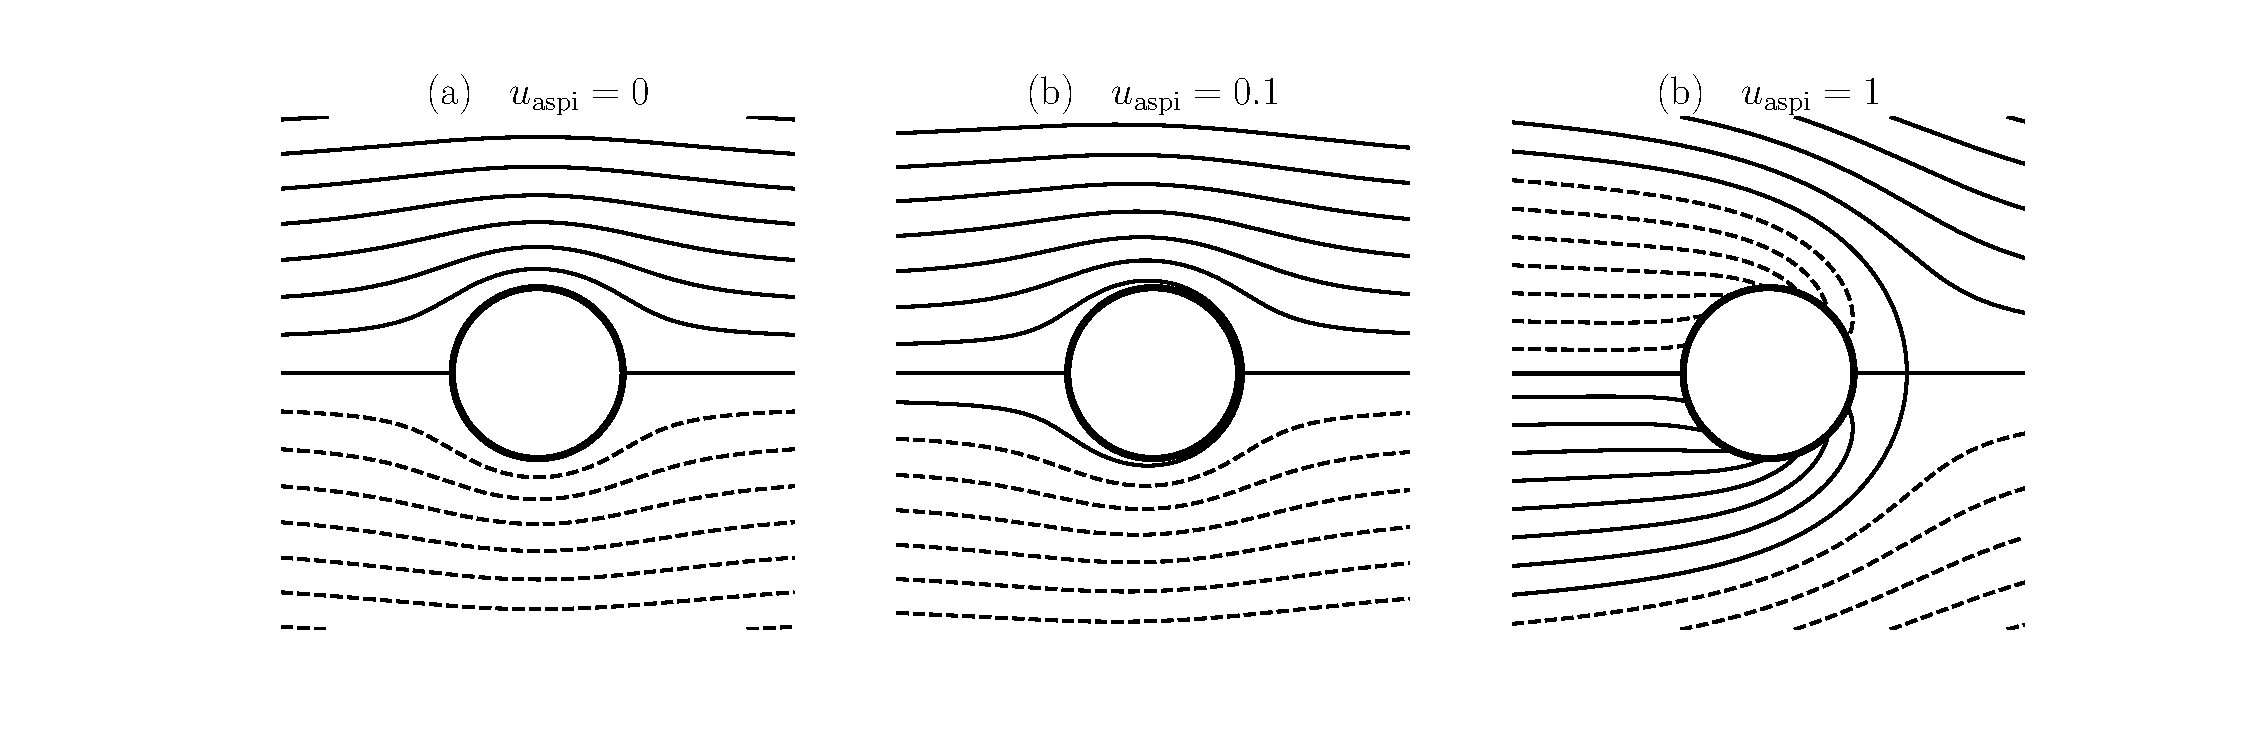
\includegraphics[width=16cm]{aspi.pdf}
      \par}
\end{answer}
\end{enumerate}
\section{Confined diffusion of a chemical species}
We aim to characterise the impact of walls or boundaries on the diffusion of a contaminant. In order to simplify the study we suppose that diffusion acts along a single axis (this may be seen as a case of translation-invariance along two directions, or of diffusion in a tube). We note $c(x,t)$ the studied concentration field.

We show that a solution to the diffusion equation
\begin{equation}
\pd{c}{t} = D \frac{\partial^2 c}{\partial x^2}
\end{equation}
that exhibit the \textit{scale invariance} property is:
\begin{equation}
c(x,t) = \frac{M}{\sqrt{4 \pi D t}} \exp\lp-\frac{x^2}{4 D t}\rp
\end{equation}
\begin{enumerate}
\item Verify that this field is actually a solution to the diffusion equation.
\item Integrate the total concentration field for a given time. What is the meaning of the constant $M$?
\item Plot with Python the evolution of this field for different instants (we'll set $M = 1$ and $D = 1$).
\end{enumerate}
\vspace{2mm}

As the diffusion equation is linear, any weight sum of elementary solutions will also be a solution. In the following we propose to use this property to build fields that comply with the boundary conditions of the problem. This approach is reminiscent of the use of ``image charges'' in electrostatics to model equipotential surfaces (boundary \textit{``metallisation''}).
\paragraph{$\rhd$ Diffusion near an impermeable wall}
A quantity $M$ of passive scalar is deposited at a distance $\ell$ from an impermeable surface located at $x = 0$. 
\begin{enumerate}[resume]
\item What is the boundary condition for the concentration field at $x = 0$ ?
\item By placing a fictitious concentration field symmetric with respect to the wall, show how to build a concentration field respecting the impermeability condition. Give the expression for this field and represent it with Python.
\end{enumerate}
\paragraph{$\rhd$ Diffusion near an absorbing wall}
We now coat the previous wall with a reactant that recombines with the concentration field so that the effective absorbing condition $c(0,t) = 0$ is now verified.
\begin{enumerate}[resume]
\item Propose a strategy to find the evolution of the concentration field in these conditions.
\item What is the concentration flux towards the wall? 
\end{enumerate}
\paragraph{$\rhd$ Confined diffusion}
We now consider the diffusion of a contaminant when confined between two impermeable walls located at $x=\pm \ell$. The contaminant is initially deposited at $x=0$.
\begin{enumerate}[resume]
\item Is it sufficient to add three elementary solutions to model the influence of the walls? To answer this question it will be helpful to estimate the flux at each wall.
\item To circumvent this issue, we propose to model the field as a superposition of an infinite sum of elementary solutions located at $x = 2 j \ell, \, j\in \mathbb{Z}$.
\item In order to determine the weight of each term, write the zero-flux condition at $x = \ell$.
\item Plot with Python the evolution of the field for different instants.
\item What is the asymptotic value of the concentration in the gap?
\end{enumerate}
\section{Liquid puddles}
 \noindent A liquid laid over a rigid substrate in the gravity field spontaneously adopts a puddle shape, as illustrated in the facing figure. The liquid has a density $\rho$, a surface tension $\gamma$ with the air, and presents a contact angle $\theta$ with the solid. We denote the gravity with $g$. 
\begin{wrapfigure}{L}{5cm}
\centering
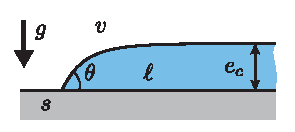
\includegraphics{flaque.pdf}
\end{wrapfigure}

\noindent We look for the limit thickness $e_c$ of the puddle far from the edges.
\begin{enumerate}
\item Represent graphically the forces acting on the puddle portion illustrated on the figure.
\item Write the equilibrium condition for the puddle, and deduce the thickness $e_c$ as a function of $\rho$, $g$, $\theta$ and $\gamma$. 
\item What is the asymptotic value of $e_c$ in the limit where $\theta \ll 1$ ?
\end{enumerate}
~

\section{Capillary adhesion of a sphere}
\begin{figure}[ht]
    \centering
    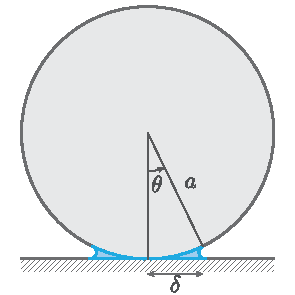
\includegraphics[valign=m,page=1]{adhesion_sphere.pdf}
    \hspace{1cm}
    \includegraphics[valign=m,page=2]{adhesion_sphere.pdf}
    \caption{\textbf{Capillary adhesion of a sphere.} Left: a sphere of radius $a$ adheres to a plane thanks to a small meniscus of radius~$\delta$. Right: the meniscus exhibits a curvature radius $r$ much smaller than the sphere radius.}
    \label{fig:adhesion}
\end{figure}
\noindent We consider in this problem the capillary adhesion undergone by a solid sphere of radius $a$ contacting a rigid plane. The sphere adhesion is induced by the presence of a small meniscus made of a perfectly wetting liquid (zero contact angle). The meniscus presents a radial extension $\delta$ that will be supposed much smaller than the radius of the sphere (see figure~\ref{fig:adhesion}). We look for a determination of the vertical component of the capillary force exercée by the meniscus on the sphere, and henceforth noted $F_\text{cap}$. We note the density $\rho$ and the surface tension of the liquid with air $\gamma$. The liquid will be considered quiescent throughout the exercise and we will neglect the influence of gravity.

\begin{enumerate}
\item Justify rapidly why the liquid viscosity cannot enter in the determination of $F_\text{cap}$. Then show using dimensional analysis that: 
$$
F_\text{cap} = \gamma a \, \mathcal F(\varepsilon),
$$
where $\varepsilon$ is a small nondimensional parameter which will be explicited. In this exercise we are interested in the limit~$\varepsilon \ll~1$.
\item As the contact angle between the liquid and the solids (both the plane and the bead) is zero, the interface is sharply curved, as indicated figure~\ref{fig:adhesion}. We suppose in particular that the curvature radius $r$ represented on the sketch is much smaller than the interface' second curvature radius. As a result we suppose that the meniscus displays a single radius of curvature $r$ in first approximation. Without calculus, give the sign of the pressure difference between the meniscus and the air $\Delta p = p_\text{ménisque} -p_\text{atm}$ ; is the meniscus in a state of higher or lower pressure with respect to the atmosphere? Explain.
\item In order to track the meniscus extension we introduce the angle $\theta$ represented on figure~\ref{fig:adhesion}. We remind that $\delta \ll a$ and therefore $\theta \ll 1$. Give the relation linking $\delta$ to $a$ and $\theta$ in first approximation.
\end{enumerate}
The force exerted by the liquid meniscus on the bead can be decomposed into two contributions: one due to Laplace pressure, and a second corresponding to the contact line action. Let's focus on the first contribution to start with. In the remaining we will not consider the influence of atmospheric pressure\footnote{In fact we can show that atmospheric pressure contribution naturally cancels out: the intensity of the adhesion force does not depend on it.}.
\begin{enumerate}[resume]
\item Noting $\mathcal S_\text{sphere}$ the portion of the sphere wetted by the meniscus, give the formal expression for the pressure force exerted by the meniscus onto the sphere.
\item Show that we can replace this expression with:
$$
\iint_{\mathcal S_\text{disc}} \!\!\!\Delta p \,\boldsymbol e_z \, \mathrm dS,
$$
where $\mathcal S_\text{disc}$ now represents the surface of the plane wetted by the meniscus.
\item On considering that $\ell \simeq 2r$ (see figure~\ref{fig:adhesion}), propose an estimation of the curvature radius $r$ as a function of $a$ and of $\theta$ to first order in  $\theta$ (we remindd that $\cos \theta = 1 - \tfrac{1}{2} \theta^2 + \tfrac{1}{24} \theta^4 + O(\theta^6)$ for $\theta \ll 1$).
\item Deduce the expression of the pressure contribution in the capillary adhesion force to first order.
\item Explain why the contact line contribution is negligible in this problem.
\item Conclude on the value of the adhesion force, and comment on the dependence with the meniscus volume. What is the limit of the function $ \mathcal F(x)$ of question 1 when $x$ tends to 0?
\end{enumerate}
\section{Curvature of a pendent drop}

\begin{wrapfigure}{L}{5cm}
\centering
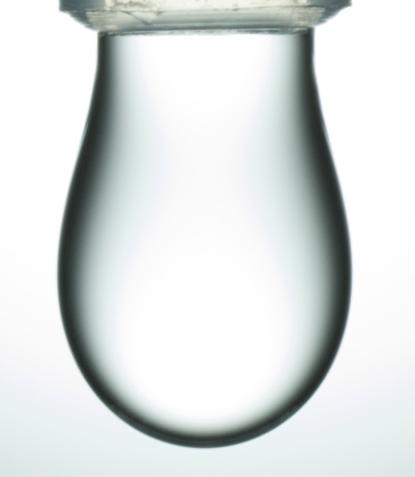
\includegraphics[width=5cm]{goutte_eau_jussieu.png}
\end{wrapfigure}
 
In order to develop a device for surface tension measurement, we wish to write a numerical code to compute the shape of an axisymmetric pendent drop.
To do so it is necessary to know the curvature $\kappa(z)$ of the drop, and to link it to the drop profile $r(z)$ (the equation for the interface is then $r = r(z)$).

\begin{enumerate}
\item Explain why working directly with $r(z)$ is not a good strategy. How does this quantity behave near the drop bottom?
\end{enumerate}
We thus work in the following with the variable $q(z) = r^2(z)$.
\begin{enumerate}
\setcounter{enumi}{1}
\item Propose a function $\mathcal S(r,z)$ that vanishes at the free surface and involves $q(z)$.
\item Compute the normalised gradient of this function. What is the meaning of this field restriction at the drop free surface?
\item Show that the drop curvature $\kappa(z)$ can be expressed as:
\begin{equation}
\kappa(z) = \frac{4 q'(z)^2 - 4q(z) (-2 + q''(z))}{(4 q(z)+q'(z)^2)^{3/2}}.
\end{equation}
\end{enumerate}

\section*{Appendix: differential operators in cylindrical coordinates}
\noindent Let $f(r,\theta,z)$ be a scalar function of space and $\boldsymbol{u}(r,\theta,z) = (u_r(r,\theta,z), u_\theta(r,\theta,z), u_z(r,\theta,z))$ a vector field. We define:
\begin{equation*}
\nabla f = \left(
\begin{array}{c}
\displaystyle\frac{\partial f}{\partial r}\\[1em]
\displaystyle\frac{1}{r}\frac{\partial f}{\partial \theta}\\[1em]
\displaystyle\frac{\partial f}{\partial z}
\end{array}
\right), 
\quad \nabla \cdot \boldsymbol{u} = \frac{1}{r} \frac{\partial}{\partial r}\bigg( r u_r\bigg) + \frac{1}{r} \frac{\partial u_\theta}{\partial \theta} + \frac{\partial u_z}{\partial z},
\quad \Delta f = \frac{1}{r} \frac{\partial}{\partial r}\bigg( r \frac{\partial f}{\partial r}\bigg) + \frac{1}{r^2} \frac{\partial^2 f}{\partial \theta^2} + \frac{\partial^2 f}{\partial z^2}
\end{equation*}

\bibliographystyle{jfm}
\bibliography{biblio_tuto}
\end{document}